% vim:ts=4:sw=4
% Copyright (c) 2014 Casper Ti. Vector
% Public domain.

\chapter{系统设计}

\section{匹配算法设计}
对于匹配算法的设计,主要的思想是探究出一种基于用户特征信息来推荐与用户志趣相投的人,所以其中必须要考虑到是现实用户对匹算算法实际效果的满意程度。之后对于不同的意见,对于匹配算法再进行不断对应的调整,从而得到一个相对最优的算法。故此,本文准备设计不同的匹配算法。之后对于不同的匹配算法进行实验,选取出实验效果最好的来当作最终实施在应用上的算法。
\subsection{基本原理}
本文所提出的匹配算法,为了
\subsection{基于人脸相似度的算法设计}

基于人脸相似度的算法设计的原理是提取用户提交的照片所提供的人脸特征,再将这一些特征与数据库中的图片的人脸特征结合起来,进行了基于算法的匹配。
face++的人脸识别所提供的特征值包括
\begin{enumerate}
\item 左眼和右眼在人脸上的相对坐标
\item 相应人脸的鼻尖在人脸上的相对坐标
\item 相应人脸的右侧嘴角和右侧嘴角在人脸上的相对坐标
\item 人脸的微笑程度分析结果,value的值为0-100的实数,越大表示微笑程度越高
\item 包含眼镜佩戴分析结果,value的值为None/Dark/Normal, confidence表示置信度
\end{enumerate}
假设一个用户提供的图片所显示的人脸为P,特征的维度为n,则用户的人靓可被定义为
\begin{equation*}
P=\{x_1,x_2,\ldots,x_n\}
\end{equation*}
设Face++提供的API的比较两张脸相似的算法为F,对于每个特征的损失函数为$L_i$,比较的人脸设为X,Y,则相似算法可表示为下式
\begin{equation*}
F=\sum_{i=1}^n L_i(x_i, y_i)
\end{equation*}
设本文的数据库的人脸集合为T,$T={T_1,T_2,\ldots}$,则我们能给出的基于人脸相似度的匹配结果的算法的公式如下
\begin{equation*}
G^{\*} = \mathop{\argmax_{G \in T}}{F(P,G)}
\end{equation*}

\subsection{机器学习算法设计}
由于基于人脸相似度的算法仅仅考虑了两个人脸特征的相似度,而基于一些美观上的经验,我们可以用过人脸的特征对于不同阶段不同年龄的人的审美进行机器学习,从而得到一个适合的算法。
但由于用户的不确定性,我们针对于用户的猜测可能导致负相关,因此这里的变量越少越好。由于现代人对于眼角位置的重视程度高于其他位置,所以在这里本文使用了眼角位置作为我们的机器学习算法所学习的变量。
\subsection{}





这一步中,用户须进行对手指点击标签和键盘输入数字的一次性设定。为了 识别输入的手指点击标签,用户须向系统提供关于大小手指点击事件的特征值。 注意到,智能手机一般是由个人拥有使用的,因此一次性设定对手机来说已经足 够充分来识别其拥有者的 TapLock 密码。



由于匹配系统不仅需要识别每个密码的键盘输入值,还需要识别每个手指点 击的二进制标签值(非大即小)。

本文将密码识别问题看做一个分类问题(或一个监督学习问题),即根据用户本身图片的特征值和过去用户感兴趣的图片信息的历史特征值来对一个手指点击事件分类。
TapLock 密码识别问题的目标是确定新发生的手指点击事件的标签(即测试 用例)。在密码设定过程中,我们收集了一组过去的手指点击事件(即训练用例), 用 D 表示这个集合。每个用例d ∈ D能被两个特征值和一个点击标签描述。令这 两个属性2为𝐴𝑑,1 = 𝑔𝑒𝑡𝑇𝑜𝑢𝑐h𝑀𝑎𝑗𝑜𝑟(), 𝐴𝑑,2 = 𝑔𝑒𝑡𝑆𝑖𝑧𝑒(),若用例 d 被分类为小(或 大)则点击标签为𝐿𝑑 = 0(或𝐿𝑑 = 1)。

\section{系统架构}
本文设计了具有如下性质的社交应用好友匹配系统。系统的服务端包括了应用Face++API的SDK程序以及连接数据库持久化存储的媒介,为用户提供对应的服务接口,并且为应用维护者提供管理和维护其数据库的方法,为用户提供查询信息以及应用匹配算法的方法
\section{服务器设计}

[用omnigraffle画一个思维导图]

\subsection{face++ SDK for node.js}
由于Face++并没有提供对应的SDK给node.js,所以本研究需要为face++的http请求的api实现一个SDK给node.js。Face++的API如下图
\begin{figure}[h]
\begin{minipage}[t]{0.45\linewidth}
\centering
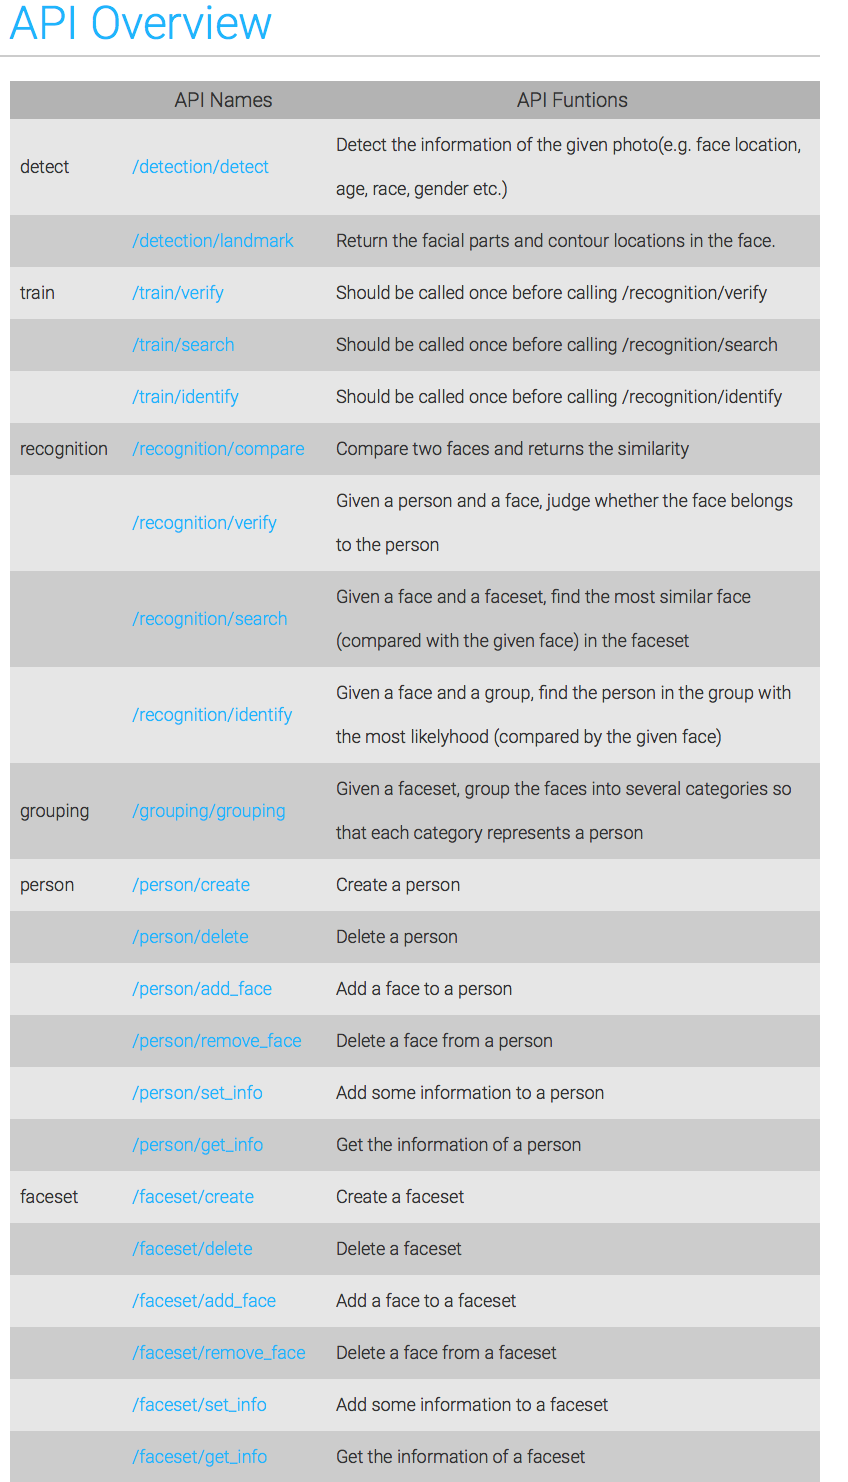
\includegraphics[width=\textwidth]{img/chap3/Face++API.png}
\caption{Face++API\label{Face++API}}
\end{minipage}
\end{figure}




\section{数据库设计}
为了完善我们的数据库的逻辑,本文对于数据库进行了ER图的描述,并用关系行数据库对于NOSQL进行了比对
[用er图]
[用mysql画的一个图]



% 中文测试文字。


